
\pagebreak

\chapter{Rozbor problematiky a~návrh řešení}
\label{navrh}
    Tato kapitola řeší celkový návrh experimentu. Od výběru zařízení pro měření a~podnětů pro vzbuzení emocí v~uživateli, přes návrh průběhu experimentu až po možné problémy, které mohou při navrhování vzniknout. Návrh lze rozdělit následovně: 
    \begin{itemize}
        \item Specifikace problému.
        \item Volba zařízení.
        \item Volba podnětů a~jejich prezentace účastníkovi experimentu.
        \item Zpracování měřených dat.
    \end{itemize}

    \section{Specifikace problému}
    \label{specifikace_problemu}
    Pro návrh experimentu je důležité určit fyziologické funkce, které budou měřeny. Nejprve je dobré se podívat, jak se již fyziologické funkce využívají v~praxi a~jak se obvykle měří. 
    
    \subsection{Využití fyziologických dat v~současné praxi}
    Z~pohledu běžného uživatele a~zlepšení jeho uživatelské zkušenosti se lze zaměřit na chytrou nositelnou elektroniku (chytré náramky, chytré hodinky). Tyto přístroje nabízí měření srdečního tepu optickými senzory (PPG snímače) a~na základě jeho variability určit typ fyzické aktivity, úroveň stresu i~kvalitu spánku (viz~\ref{srdecni_tep}). Již však neposkytují podrobnější informace o~emočním stavu člověka, který je pro jeho zdraví i~uživatelskou zkušenost významný.
    
    Jako další pohled na problematiku se nabízí proces testování uživatelských rozhraní. V~této fázi vývoje se často využívají metody, mezi které patří dotazníky, monitorování pohybu očí (viz~\ref{eye_tracking}), monitorování pohybu myší apod. Žádná z~těchto metod neumožňuje přímou detekci emocí uživatele a~je nutné se spoléhat na jeho zpětnou vazbu, která může být zkreslená.
    
    \subsection{Definice zaměření práce}
    Z~těchto důvodu jsem se ve své práci zaměřil na emotivitu člověka a~její vliv na fyziologické funkce. Při návrhu budu vycházet z~dřívějších studií, které jsou popsány v~podkapitole~\ref{emotion_to_physio}. Cílem je stimulovat autonomní nervový systém (popsán v~podkapitole~\ref{nervous_system}) dobrovolníků tak, aby postupně pociťovali různé emoce a~měřit jejich projevy za pomocí obvyklých senzorů používaných v~chytré nositelné elektronice pro měření fyziologických dat.
    
     
    \section{Volba zařízení a~měřených metrik}
    \label{volba_zarizeni_metriky}
    Jak je popsáno v~podkapitole~\ref{popis_dat_mereni}, fyziologické funkce je možné měřit více způsoby. Základní rozdělení metod je na invazivní a~neinvazivní. Výhodou invazivní oproti neinvazivní metodě jsou bezesporu přesnější data. Na druhou stranu je jejich použití nepohodlné a~pro běžné užití nevhodné. Proto jsem se zaměřil na neinvazivní metody.
    
    Základní měřenou funkcí lze označit \textbf{srdeční tep} (viz~\ref{srdecni_tep}), jenž je možné měřit dvěma metodami. Pomocí EKG přístroje, nebo optickými snímači. EKG přístroje nabízí přesnější a~podrobnější data, nicméně jsou stále více využívány optické snímače. Důvodem je snadnější technická realizace i~cena. 
    
    Z~dalších fyziologických funkcí, jako je měření krevního tlaku, dýchání, galvanické odezvy kůže, měření oční aktivity apod., se nabízí jako nejméně rušivé pro uživatele, měření \textbf{galvanické odezvy kůže} (viz~\ref{gsr}).
    
    S~určenými funkcemi, které budou měřeny, lze vybrat zařízení pro jejich měření. Je možné využít pro každou metriku specifické zařízení a~nebo využít zařízení disponující všemi potřebnými snímači. Pro měření fyziologických dat jsem, na základě doporučení vedoucího práce, zvolil náramek E4 společnosti Empatica. 
    
    \subsection{Empatica E4}
    \label{empatica_e4}
     Jedná se o~zdravotnické nositelné zařízení umožňující sledovaní fyziologických dat v~reálném čase, jejich snadné zpracování, analýzu a~vizualizaci~\cite{e4}. Podstatné vlastnosti zařízení:
        \begin{multicols}{2}
            \begin{itemize}
                \item Snadný přístup k~datům a~pokročilá vizualizace.  
                \item Kvalita a~přesnost měření.
                \item Certifikované zařízení\footnote{\url{https://www.emergobyul.com/services/europe/ce-certification}}. 
                \item Snadné a~nerušivé měření.
                \item API\footnote{\url{https://cs.wikipedia.org/wiki/API}} umožňující tvorbu vlastních aplikací.
                \item PPG senzor\footnote{\url{https://en.wikipedia.org/wiki/Photoplethysmogram}}, GSR (EDA\footnote{\url{https://en.wikipedia.org/wiki/Electrodermal_activity}}) senzor, senzor teploty kůže, akcelerometr
                \item Tlačítko pro značení událostí v~signálech.
            \end{itemize}
        \columnbreak
            \begin{figure}[H]
                \centering
                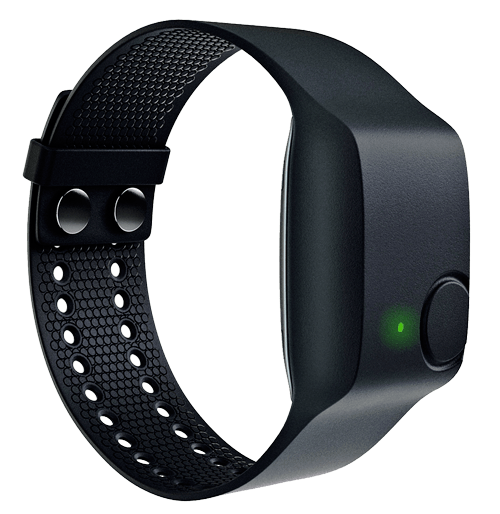
\includegraphics[scale=0.3]{obrazky-figures/e4-front_light.png}
                \caption{Náramek E4 společnosti Empatica.}
                \label{fig:e4_fig}
            \end{figure}    
        \end{multicols}
        
        
        Zařízení již bylo využito v~několika studiích. Příkladem může být studie~\cite{e4_validation}, ve které bylo ověřováno, zda data získaná pomocí PPG senzoru náramku jsou dostatečně kvalitní pro odhalení srdečních poruch. Data byla porovnávána s~daty získanými ECG senzory. Data z~náramku E4 byla častěji chybná, avšak ve více než 85\,\% byla data stejně kvalitní. Nutno podotknout, že byly použity 3~ECG senzory v~porovnání s~jedním PPG senzorem. Experiment byl proveden se 7 účastníky.
        
        Další studie~\cite{e4_reliability} zkoumala spolehlivost náramku Empatica E4 pro měření elektrodermální aktivity na emoční podněty. Pro porovnání byl použit laboratorní systém Refa\footnote{Twente Medical Systems International B.V., Zutphenstraat, Nederland, odkaz: \url{https://www.tmsi.com}}. Cílem experimentu bylo detekovat změny v~EDA pro pozitivní, negativní a~neutrální vizuální podněty. Experimentu se zúčastnilo 59 dobrovolníků. Předpokladem, na základě předešlých studií, byl vzrůst EDA pro pozitivní i~negativní podněty a~pokles pro neutrální podněty. Hodnoty získané systémem Refa odpovídaly předpokladům pro pozitivní a~neutrální podněty. Zařízení E4 potvrdilo předpoklady pro pozitivní a~negativní podněty. Pro neutrální podněty E4 žádné změny nezaznamenala. Důvodem může být nízká frekvence senzoru EDA (4\,Hz).
        
        Zda náramek poskytuje dostatečně kvalitní data pro detekci stresu ověřovala studie \cite{e4_stress_detection}, kde byl využit jak EDA senzor, tak PPG senzor. Experiment byl založen na laboratorním testu \uv{Trier Social Stress Test}\footnote{\url{https://www.ncbi.nlm.nih.gov/pmc/articles/PMC5314443/}}. Testovací skupina byla tvořena 7~lidmi. V~porovnání s~dalšími senzory, signál z~PPG senzoru vykazoval značnou chybovost. Příčinou chybovosti bylo příliš velké zašumění vlivem vnějších vlivů (pohyb ruky, špatný kontakt apod). Chybovost se projevila především při získávání variability srdečního tepu. Naopak hodnoty průměrného srdečního tepu nebyly příliš ovlivněny. Dále se ukázalo, že EDA senzor poskytuje kvalitní a~spolehlivá data.
        
        \vspace{3mm}
        
        Ze studií vyplývá, že zařízení ne vždy poskytuje kvalitní data a~je nutné počítat s~jistými limity. Ty z~velké části vychází z~technických omezení (nevýhody PPG senzoru jsou popsány v~podkapitole~\ref{srdecni_tep}) použitých technologií. Na druhou stranu jsou případy, kdy dokáže produkovat data kvalitnější než jiná zařízení.
        
        \subsubsection{Komunikace se zařízením}
        Zvolené zařízení nabízí více možností komunikace pro přenos dat. V~případech, kdy by bylo nepraktické, nebo dokonce nemožné být v~blízkosti počítače, či mít v~blízkosti mobilní zařízení, nabízí možnost nahrávacího módu. Nevýhodou je především pracné stahování dat ze zařízení a~omezená délka nahrávání kapacitou vnitřního úložiště. 
        
        \begin{figure}[H]
            \centering
            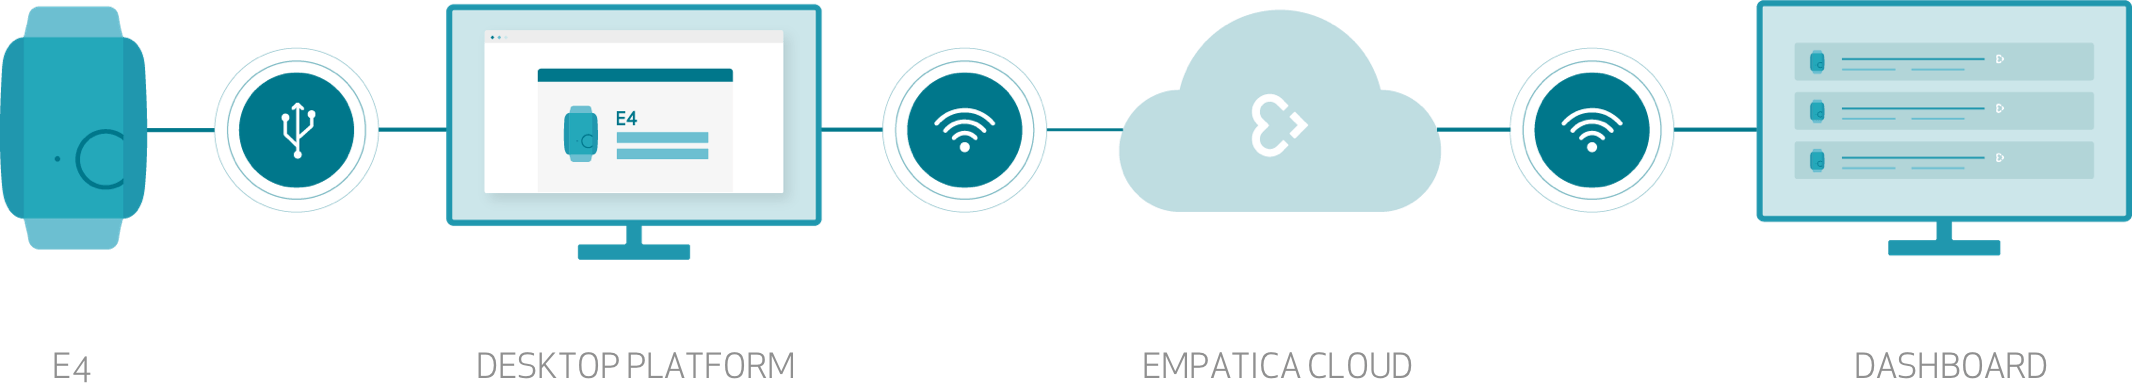
\includegraphics[width=\textwidth]{obrazky-figures/e4-recording_system.png}
            \caption{Schéma pro nahrávání dat do vnitřní paměti zařízení a~následné získání dat.}
            \label{fig:recording_fig}
        \end{figure}
        
        Nejčastěji používaná je metoda streamování v~reálném čase. Pro tuto metodu je nutný chytrý mobilní telefon s~aplikací od společnosti Empatica. Výhodou je základní vizualizace dat v~mobilní aplikaci a~automatické nahrávání dat do cloudu společnosti Empatica. Mezi nevýhody patří automatické odpojení a~vypnutí zařízení po každém nahrávání. 
        
        \begin{figure}[H]
            \centering
            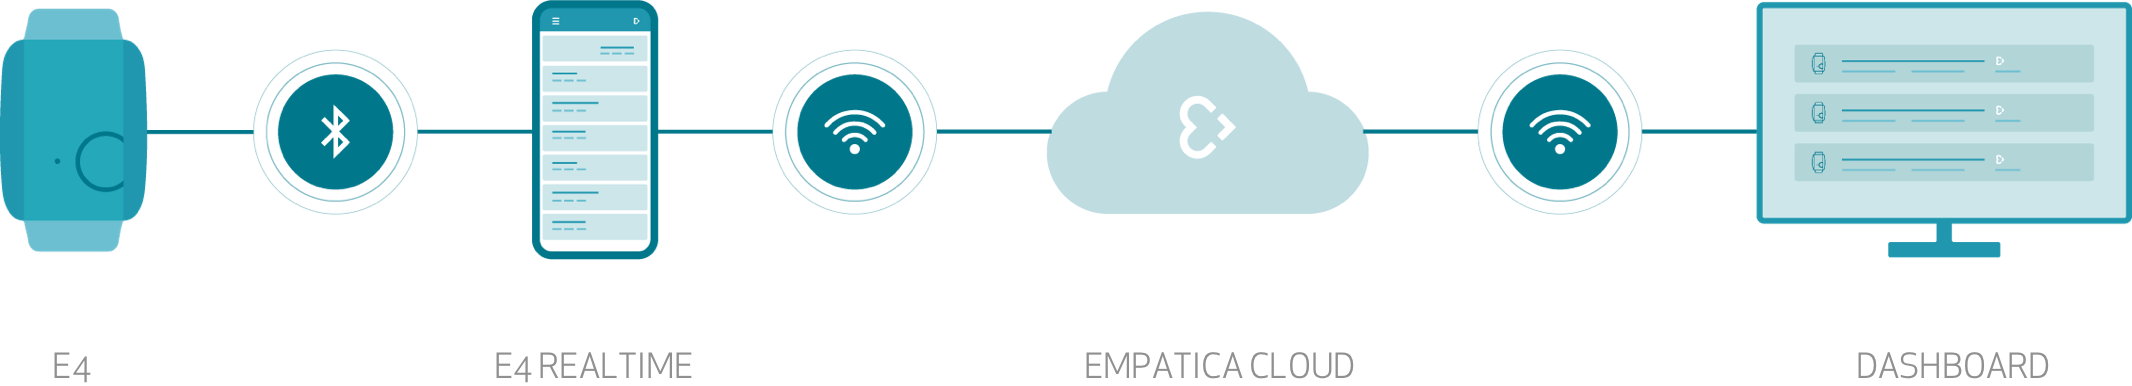
\includegraphics[width=\textwidth]{obrazky-figures/e4-streaming_system.png}
            \caption{Schéma real--time komunikace. Data jsou streamována do mobilní aplikace a~následně uložena do cloudu.}
            \label{fig:stream_fig}
        \end{figure}
        
        Třetí metoda je určena především pro vývojáře vlastních aplikací. Pro komunikaci je nutné implementovat vlastního TCP klienta\footnote{\url{https://cs.wikipedia.org/wiki/Transmission_Control_Protocol}}. Dále je nutné zakoupit Bluetooth zařízení BLED112\footnote{\url{https://www.silabs.com/wireless/bluetooth/bluegiga-low-energy-legacy-modules/device.bled112}}. Mezi výhody patří možnost definovat sledované typy dat (galvanická odezva kůže, srdeční tep, teplota, stav baterie, časové značky). Tato metoda jediná umožňuje streamování dat bez opětovného zapínání náramku po skončení předešlého sezení.
    
        \vspace{3mm}
        
        \begin{figure}[H]
            \centering
            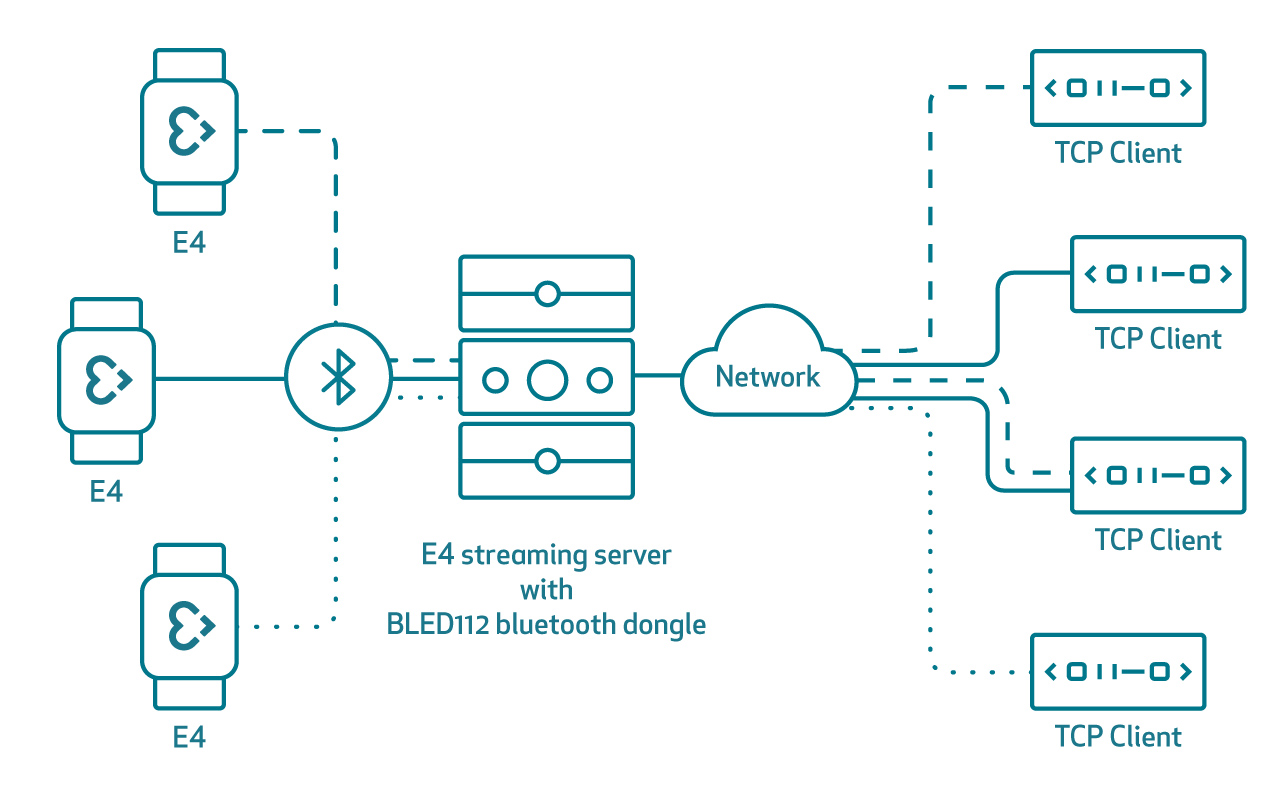
\includegraphics[scale=0.4]{obrazky-figures/E4_streaming_server_scheme.png}
            \caption{Schéma komunikace pomocí E4 streamovacího serveru. Na levé straně zobrazuje jednotlivé E4 náramky připojené pomocí BLED112 Bluetooth zařízení k~počítači. Na pravé straně ilustruje TCP klienty, přes které lze získávat data. Jednotlivé druhy čar zobrazují datový tok mezi zařízeními.}
            \label{fig:server_fig}
        \end{figure}
    
    \section{Volba podnětů}
    \label{podnety_volba}  
    
    Pro volbu podnětů a~tvorbu vhodné datové sady je důležité, aby byla zachována objektivita zvolených stimulů, nicméně je neméně podstatné brát v~potaz také individualitu člověka. Obecně je vhodné se zaměřit na typické podněty. Příkladem může být obrázek roztomilého štěněte vzbuzující příjemné pocity. Na základě předešlých studií (viz podkapitola~\ref{emotion_to_physio}), lze uvažovat tyto kategorie:
    \begin{itemize}
        \item obrázky,
        \item zvuky,
        \item videa,
        \item aktivní činnost (práce s~uživatelským prostředím, plnění úkolu na čas),
        \item počítačové hry.
    \end{itemize}
    
    Uvažujme případ, kdy by bylo cílem experimentu dostat účastníka do stresové situace, při které by byly pozorované události: klidový stav, stresový stav, případně vliv únavy na řešení úkolu. V~takovém případě se jeví jako vhodné využít úkoly různé obtížnosti, na jejichž splnění by byl stanovený čas. Jelikož je však tato práce zaměřena více na jednotlivé emoce, není tento typ experimentu vhodný. Základním předpokladem vyvolání emoce u~člověka je zážitek spojený s~událostí, či jakkoliv zachycenou (vizuálně, zvukově) situací (viz. \ref{emotivita}). 
    
    Podobné problémy též provází použití počítačových her jako stimulu. Neboť není zaručeno, jakou emoci a~především kdy hráč (účastník experimentu) pocítí. V~potaz je také nutné brát lidský faktor (individuální obliba účastníků hraní počítačových her) i~časovou náročnost experimentu.  
    
    Jako nejvhodnější řešení se tedy jeví využití obrázků, zvuků, či videí. Tyto typy podnětů dovolují přesně definované časové úseky promítání, variabilitu kombinací podnětů i~poměrně malou časovou náročnost experimentu. Navíc, díky možnosti vytvoření přesného schématu, usnadňují zpracování získaných dat. Pro vzbuzení emocí je důležitá správná volba a~kombinace těchto podnětů. Na základě vědeckých studií jsou k~dispozici databáze, jenž obsahují obrázky s~patřičným skóre určujícím typ emoce, který vyvolávají. Pro kategorizaci se využívá hodnota míry pozitivity a~síla vzrušení. Kategorizace je popsána v~podkapitole \ref{emotivita}. Volba databáze pro experiment závisí na výběru sledovaných emocí. Příkladem mohou být tyto:
    \begin{itemize}
        \item Categorized Affective Pictures Database (CAP-D) \cite{CAP-D},
        \item DIsgust-RelaTed-Images (DIRTI) database \cite{DIRTI},
        \item Geneva Affective Picture Database (GAPED) \cite{gaped},
        \item Set of Fear Inducing Pictures (SFIP) \cite{SFIP},
        \item Socio-Moral Image Database (SMID) \cite{SMID},
        \item Open Affective Standardized Image Set (OASIS) \cite{oasis}.
    \end{itemize}
    
     Výhodou použití těchto databází je široká škála volně využitelných obrázků, jenž byly kategorizovány na základě širokého průzkumu. Pro doplnění lze využít také obrázky, zvukové stopy a~videonahrávky z~veřejných online zdrojů (Pexels\footnote{\url{https://www.pexels.com}}, SoundBible\footnote{\url{https://soundbible.com}}, Zapsplat\footnote{\url{https://www.zapsplat.com}}, Mazwai\footnote{\url{https://mazwai.com}}, apod.) pod licencí \emph{Creative Commons}\footnote{\url{https://creativecommons.org/licenses/by/3.0/cz/}}. Podněty jsou uspořádány do prezentací, které budou promítány dobrovolníkům pro experiment. Při vytváření bylo zvažováno více kombinací těchto podnětů a~jejich uspořádání. 
    
    Jako první řešení se nabízí náhodná kombinace a~posloupnost obrázků. Tuto prezentaci promítnout dobrovolníkům a~počkat na jejich zpětnou vazbu, podle které pak kategorizovat získaná data. Tento postup je obvyklý. Při navrhování jsem z~této metody vycházel a~postupně na ni aplikoval následující úpravy. Cílem těchto úprav je snaha minimalizovat prolínání emocí a~zvýšit fyziologickou odezvu na podněty.
    
    \textbf{1.\,úprava} vkládá mezi jednotlivé podněty neutrální obrazy, jenž umožní uklidnění emocí dobrovolníka, čímž se sníží vliv předchozí emoce na současnou emoci a~tím zpřesnění naměřených dat. Tato úprava se běžně využívá (viz podkapitola \ref{emotion_to_physio}).
    \begin{figure}[H]
        \centering
        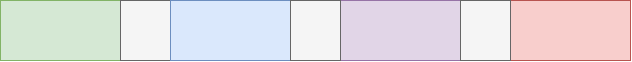
\includegraphics[width=\textwidth]{obrazky-figures/podnety_jine_emoce.png}
        \caption{Schéma posloupnosti podnětů vzbuzující různé emoce v~krátkém časovém intervalu při aplikaci 1.\,úpravy (šedé zóny). Každá barva značí jinou emoci.}
        \label{fig:podnety_jine_emoce}
    \end{figure}
    
    \textbf{2.\,úprava} ještě více eliminuje prolínání emocí a~také rozšiřuje získanou datovou sadu pro jednotlivé emoce. Jelikož musí být datová sada objektivní, není zaručeno, že zvolený vizuální stimul vzbudí v~člověku emoci. Nabízí se tedy možnost vytvořit více prezentací, kde každá prezentace bude obsahovat podobné obrazy s~podobným kategorizačním skóre. Tím se zvýší pravděpodobnost vzbuzení emoce dobrovolníka podstupujícího experiment.  
    
    \begin{figure}[H]
        \centering
        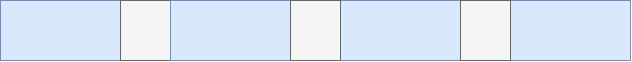
\includegraphics[width=\textwidth]{obrazky-figures/podnety_schema.png}
        \caption{Aplikace 2.\,úpravy na posloupnost podnětů.}
        \label{fig:podnety_schema}
    \end{figure}
    
    \textbf{3.\,úprava} by měla zvýšit pravděpodobnost vzbuzení emoce i~zvýšení míry její intenzity. Jak je popsáno v~sekci \ref{nervous_system}, vizuální a~zvukové podněty tvoří převážnou většinu vjemů v~každodenním životě člověka, díky čemuž je zajímavé využít jejich kombinaci. 
    
    Při aplikaci všech těchto úprav vzniká schéma prezentace zobrazeno na obr.\,\ref{fig:podnety_ruzna_intenzita}. Pro vzbuzení intenzivnější emoce a~tím zlepšení získaných dat, jsou použity statické obrázky, zvukové stopy i~videonahrávky.
    
    \begin{figure}[H]
        \centering
        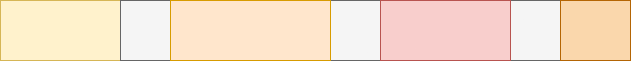
\includegraphics[width=\textwidth]{obrazky-figures/podnety_ruzna_intenzita.png}
        \caption{Schéma posloupnosti podnětů vzbuzující stejné emoce v~krátkém časovém intervalu v~různé intenzitě pomocí kombinace zvukových a~vizuálních stimulů i~různé délky doby stimulace. Různost odstínu barev značí různé kombinace podnětů.}
        \label{fig:podnety_ruzna_intenzita}
    \end{figure}
    
    V~případě využití popsaného schématu pro experiment vzniká problém označení jednotlivých epoch. Jako řešení se nabízí použití spínače, který bude stisknut v~odpovídajících časech vzhledem k~průběhu prezentace. Fyzický spínač může být konkrétní klávesa na klávesnici, nebo externí spínač připojený k~počítači. Jelikož je pro experiment zvoleno zařízení Empatica E4, které obsahuje vlastní tlačítko umožňující vysílat časové značky při stisku, je tento problém poměrně snadno vyřešen.
    
    \vspace{3mm}
    
    Dalším krokem je stanovení emocí, na které experiment cílí. V~podkapitole \ref{emotivita} bylo stanoveno 7~základních emocí, jenž jsou snadno rozpoznatelné. Obvykle postačuje výraz v~obličeji. Z~těchto základních dále vychází odvozené emoce, které jsou více specifické (úzkost, empatická bolest, touha apod.), zato hůře rozpoznatelné. Samotným problémem je také vzbuzení takto konkrétních emocí pomocí omezené datové sady v~krátkém časovém horizontu s~ohledem na individualitu člověka. Zaměřil jsem se tedy pouze na emoce základní.
    
    
    \section{Přijímání a~zpracování měřených dat}
    Jak je specifikováno výše, práce se soustředí na měření fyziologických funkcí v~závislosti na emocích člověka. Pro získávání těchto dat bylo vybráno zařízení Empatica E4. Z~důvodu automatizace a~snadnějšího následného zpracování dat jsem zvolil komunikaci se zařízením pomocí streamovacího serveru. Tento způsob vyžaduje stažení serveru ze stránek společnosti Empatica určených pro vývojáře\footnote{\url{https://developer.empatica.com/windows-streaming-server-usage.html}}. Server je dostupný pouze pro operační systém Windows. 
    
    \subsection{Příjem dat}
    Komunikace probíhá pomocí TCP klienta a~je nutné jej implementovat. Jelikož server umožňuje připojení více zařízení najednou, tak je důležité specifikovat jednoznačné ID zařízení, jenž je přidělené výrobcem. Po připojení implicitně vysílá zařízení data získaná ze všech senzorů včetně stavu baterie. Jednotlivé kanály lze vypnout pomocí kontrolních zpráv zaslaných na server. Kontrolní zprávy mají definované schéma následovně: <PŘÍKAZ> <SEZNAM ARGUMENTŮ>. Přijímání dat probíhá neustále, dokud není spojení ukončeno, nebo pozastaveno kontrolní zprávou. Server vysílá dva typy zpráv. Prvním typem jsou informační zprávy, které obsahují informace o~stavu spojení, či obsahují odpovědi na kontrolní zprávy zaslané na server. Schéma těchto zpráv je stejné jako u~kontrolních zpráv. Pro odlišení začínají písmenem~\uv{R}. Druhým typem jsou datové zprávy. Datové zprávy jsou vysílány ve tvaru: <TYP SIGNÁLU> <ČASOVÁ ZNAČKA> <DATA>. Blíže je protokol zpráv popsán na webových stránkách výrobce\footnote{\url{https://developer.empatica.com/windows-streaming-server-commands.html##protocol-example}}.
    
    \subsection{Zpracování dat}
    Získaná data jsou neuspořádaná a~v~nevhodném formátu. Dalším krokem je tedy rozdělení dat podle typu signálu. Každý signál obsahuje data ve formátu: <ČASOVÁ ZNAČKA> <HODNOTA>. Při zpracování je vhodné provést normalizaci časových značek. Tento proces je prováděn, neboť časové značky vysílané zařízením obsahují data ve formátu UNIXového času\footnote{Počet sekund od (UTC) 00:00:00 1.\,ledna 1970}. Normalizace je provedena pomocí datové zprávy s~nejnižší hodnotou časové značky, typicky první záznam v~souboru dat. Výsledný formát dat vypadá následovně: <ČASOVÁ ZNAČKA> <HODNOTA> <NORMALIZOVANÁ ČASOVÁ ZNAČKA>. Normalizovaná časová značka může usnadnit orientaci v~datech při zpracování dat (např. přehlednější vizualizace, manuální kontrola).
    
    \subsection{Extrakce příznaků}
    Uspořádaná data pro jednotlivé signály je možné dále zpracovat za účelem extrakce příznaků signálů. Tyto příznaky lze následně využít pro strojové učení. Sledované signály a~jejich podstatné příznaky jsou popsány v~kapitole \ref{popis_dat_mereni}. Jako vhodný programovací jazyk se jeví jazyk Python\footnote{\url{https://www.python.org}} s~využitím knihovny Pandas\footnote{\url{https://pandas.pydata.org}}, či SciPy\footnote{\url{https://www.scipy.org}}. Ačkoliv se knihovna SciPy obecně využívá pro zpracování signálů, tak pro zpracování fyziologických dat existují specializované knihovny, popsané v~sekci~\ref{navrh_implementace}, jenž z~této knihovny vychází. 
    
    Vstupní signál celého procesu typicky obsahuje nežádoucí šum (nízkofrekvenční, vysokofrekvenční), který je nutné filtrovat. Tím vznikne čistý signál vhodný pro zpracování. Signály jsou typicky vysílány v~různých frekvencích v~závislosti na použitém senzoru. Senzory E4 vysílají data v~těchto frekvencích: GSR: 4\,Hz, PPG: 64\,Hz, Akcelerometr: 32\,Hz, Teplota kůže: 4\,Hz. Proto je nutné jednotlivé signály převzorkovat tak, aby byla frekvence požadovaných signálů i~délka datových souborů stejná (původní signály jsou zachovány). Na fyziologické signály je obvykle nahlíženo nikoliv jako na jeden celek, ale jako na časové úseky, které obsahují odezvu autonomní nervové soustavy na stimul. Další zpracování tedy může probíhat dvěma způsoby. První možností je zpracovávat signál v~jednotlivých časových oknech označených explicitně časovými značkami ze spínače náramku E4. Dalším způsobem je využít tzv. \textbf{klouzavé okno}~\cite{sliding_window}. Šířka klouzavého okna je proměnná a~určuje, která složka signálu (frekvenční, časová) je lépe rozlišitelná. Široké okno poskytuje lepší frekvenční rozlišení, ale špatné rozlišení časové složky. Opakem je úzké okno. Dalším kritériem je krok posouvání okna. Obecně lze říci, čím menší krok je a~tím je větší překrytí vzorků, tím je dosaženo lepších výsledků za cenu vyšší časové náročnosti. 
    
    Fyziologické funkce jsou ovlivněny aktuálním stavem člověka a~klidový stav je velmi individuální. Proto není možné porovnávat signály v~jednotlivých časových oknech s~jedním obecným signálem klidového stavu. Pro každého účastníka musí být určen minimálně jeden výchozí signál klidového stavu. Samotný experiment však mění aktuální stav účastníka a~tím mění i~jeho fyziologické funkce v~klidovém stavu. Proto je výchozí signál měřen vícekrát. 
    
    \subsection{Implementace}
    \label{navrh_implementace}
    Celý proces zpracování signálů je možné implementovat od základu. Avšak není to nutné, neboť existují již specializované knihovny. Jejich výběr určuje především typ i~průběh experimentu. Dalším kritériem jsou zvolené metriky. Nejlépe odpovídající knihovny navrženému experimentu jsou knihovna \emph{pyphysio}~\cite{pyphysio} a~\emph{NeuroKit2}~\cite{Makowski2021neurokit}. Obě knihovny obsahují pokročilé nástroje pro zpracování všech typů měřených signálů. 
    
    \vspace{6mm}
    
    \section{Shrnutí návrhu řešení}
    Během návrhu bylo specifikováno zaměření experimentu, kdy půjde o~pokus vzbudit v~člověku různé typy emocí a~následně měřit jejich vliv na fyziologické funkce. Návrh vychází z~dosavadních studií (podkapitola~\ref{emotion_to_physio}). Pro měření byl zvolen náramek Empatica E4. Pozorované fyziologické funkce byly zvoleny tyto: srdeční tep, galvanická odezva kůže. Zaznamenány jsou i~další data vysílané zařízením vyjma akcelerometru. Data akcelerometru nejsou zaznamenány, neboť je účastník po celou dobu v~klidové poloze a~nedochází k~žádnému pohybu.  Dále byly popsány možné podněty a~jejich schéma promítání, kde po krátké úvaze byly zvoleny obrázky, zvuky a~videonahrávky. Poslední část návrhu byla věnována zpracování získaných dat, kde byly probrány podstatné kroky k~extrakci příznaků i~možné knihovny využitelné k~implementaci. Nakonec byl zvolen pro implementaci jazyk Python. Jako potenciální knihovny byly navrženy Pandas, pyphysio a~NeuroKit2.
